\documentclass[a4paper, 12pt]{article}%тип документа

%%%Библиотеки
	%\usepackage[warn]{mathtext}	
	\usepackage[T2A]{fontenc} % кодировка
	\usepackage[utf8]{inputenc} % кодировка исходного текста
	\usepackage[english,russian]{babel} % локализация и переносы
	\usepackage{caption}
	\usepackage{listings}
	\usepackage{amsmath,amsfonts,amssymb,amsthm,mathtools}
	\usepackage{wasysym}
	\usepackage{graphicx}%Вставка картинок правильная
	\usepackage{float}%"Плавающие" картинки
	\usepackage{wrapfig}%Обтекание фигур (таблиц, картинок и прочего)
	\usepackage{fancyhdr} %загрузим пакет
	\usepackage{lscape}
	\usepackage{xcolor}
	\usepackage[normalem]{ulem}
	\usepackage{hyperref}

%%%Конец библиотек




%%%Настройка ссылок
	\hypersetup
	{
		colorlinks=true,
		linkcolor=blue,
		filecolor=magenta,
		urlcolor=blue
	}
%%%Конец настройки ссылок


%%%Настройка колонтитулы
	\pagestyle{fancy}
	\fancyhead{}
	\fancyhead[L]{Вопрос по выбору}
	\fancyhead[R]{Талашкевич Даниил, группа Б01-009}
	\fancyfoot[C]{\thepage}
%%%конец настройки колонтитулы



							\begin{document}
						%%%%Начало документа%%%%


%%%Начало титульника
\begin{titlepage}

	\newpage
	\begin{center}
		\normalsize Московский физико-технический институт \\(госудраственный 			университет)
	\end{center}

	\vspace{6em}

	\begin{center}
		\Large Лабораторная работа по электричеству\\
	\end{center}

	\vspace{1em}

	\begin{center}
		\large \textbf{Свободные колебаний в электрическом контуре [3.2.4]}
	\end{center}

	\vspace{2em}

	\begin{center}
		\large Талашкевич Даниил Александрович\\
		Группа Б01-009
	\end{center}

	\vspace{\fill}

	\begin{center}
	Долгопрудный \\2021
	\end{center}
	
\end{titlepage}
%%%Конец Титульника



%%%Настройка оглавления и нумерации страниц
	\thispagestyle{empty}
	\newpage
	\tableofcontents
	\newpage
	\setcounter{page}{1}
%%%Настройка оглавления и нумерации страниц


					%%%%%%Начало работы с текстом%%%%%%

\section{Аннотация}

\subsection{Цель работы}
\begin{enumerate}
\item   Исследование свободных колебаний в электрическом контуре.
\end{enumerate}

\subsection{В работе используются:}
\begin{itemize}
    \item Генератор импульсов
    \item электронное реле
    \item магазин сопротивлений
    \item магазин емкостей
    \item катушка индуктивности
    \item электронный осциллограф
    \item универсальный измерительный мост 

\end{itemize}

\subsection{Теоретическое вступление и модель}

В работе планируется:

\begin{enumerate}
    \item Исследовать зависимость периода свободных колебаний контура от емкости. Согласно теории, зависимость должна иметь вид (Формула Томпсона):

\begin{equation}
    T = 2\pi \sqrt{LC} \quad
\end{equation}
    

    где $T$ - период колебаний, $L$ и $C$ - индуктивность и емкость контура соответственно.

    Период планируется измерять с помощью осциллографа.

    \item Исследовать зависимость логарифмического декремента затухания от сопротивления. \\ Расчет логарифмического декремента затухания будет производиться по следующей формуле:

\begin{equation}
	\lambda = \frac{1}{n} \ln\frac{W_k}{W_{k+n}} \quad    
\end{equation}
    

    где $W_i$ - энергия контура после i-того колебания.

    Энергию контура планируется высчитывать используя напряжение на конденсаторе, которое в свою очередь, измеряется с помощью осциллографа. \\

    
Согласно теории, логарифмический декремент затухания пропорционалени сопротивлению
\begin{equation}
	\lambda \propto R
\end{equation}
    
    \newpage

    \item Определить критическое сопротивление. Критическое сопротивление вычисляется по формуле:

\begin{equation}
	R_\text{кр} = 2\sqrt{\frac{L}{C}}
\end{equation}
   

    \item Определить добротность контура. Добротность планируется вычислить двумя способами, с последующим сравнением результатов. \\

    Первый способ - Через формулу для логарифмического декремента затухания. \\
    Второй способ - используя параметры контура R, L, C. \\[0.1cm]

    Формула для вычисления добротности через логарифмический декремент затухания:
\begin{equation}
	Q = \frac{\pi}{\lambda}
\end{equation}
    Формула для вычисления добротности с использованием параметров контура
\begin{equation}
 	Q = \frac{1}{R} \sqrt{\frac{L}{C}}
\end{equation}

\end{enumerate}

\section{Экспериментальная установка}

Схема установки представлена на рисунке 1.

\begin{center}

    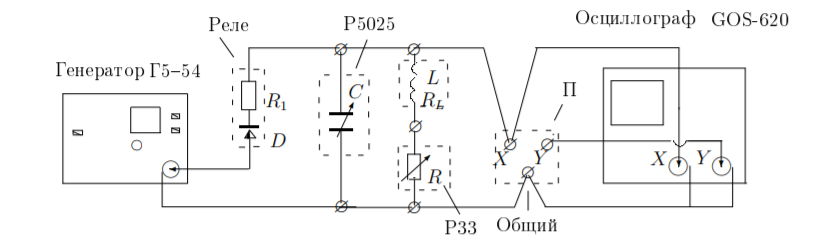
\includegraphics[scale=0.6]{324_scheme.png} \\
    \textit{Рис. 1. Схема установки}

\end{center}

\section{Ход работы}

После совершения всей предварительной настройки оборудования: сборки схемы, настройки осциллографа и т.п., мы можем наблюдать картину затухающих колебаний  

Прежде всего измерим индуктивность $L$ и сопротивление катушки $R_L$ в зависимости от частоты 

\begin{table}[h!]
\begin{center}

\begin{tabular}{|c|c|c|}
\hline
$\nu$, Гц & $L$, мГн & $R_L$, Ом \\ \hline
50        & 200,4    & 11,1      \\ \hline
1000      & 200,1    & 18,8      \\ \hline
5000      & 200,4    & 41,2      \\ \hline
\end{tabular}
\caption{Некоторые параметры катушки индуктивности}
\end{center}
\end{table}
В итоге мы получаем, что $L = 200 \pm 0,2$ мГн.
\newpage

\subsection{Подготовка}

Проделав всю подготовительную работу: полная настройка осциллографа, разобраться с его работой, сборка схемы, настройка емкостного магазина вместе с магазином сопротивлений, мы можем приступать к основной части работы.

\subsection{Измерение периодов свободных колебаний}

Установим на магазине сопротивлений $R = 0$ Ом и $C = 0,02$ мкФ. Подобрав частоту развертки получим изображение наших колебаний на осциллографе:

\begin{figure}[h!]
\begin{center}
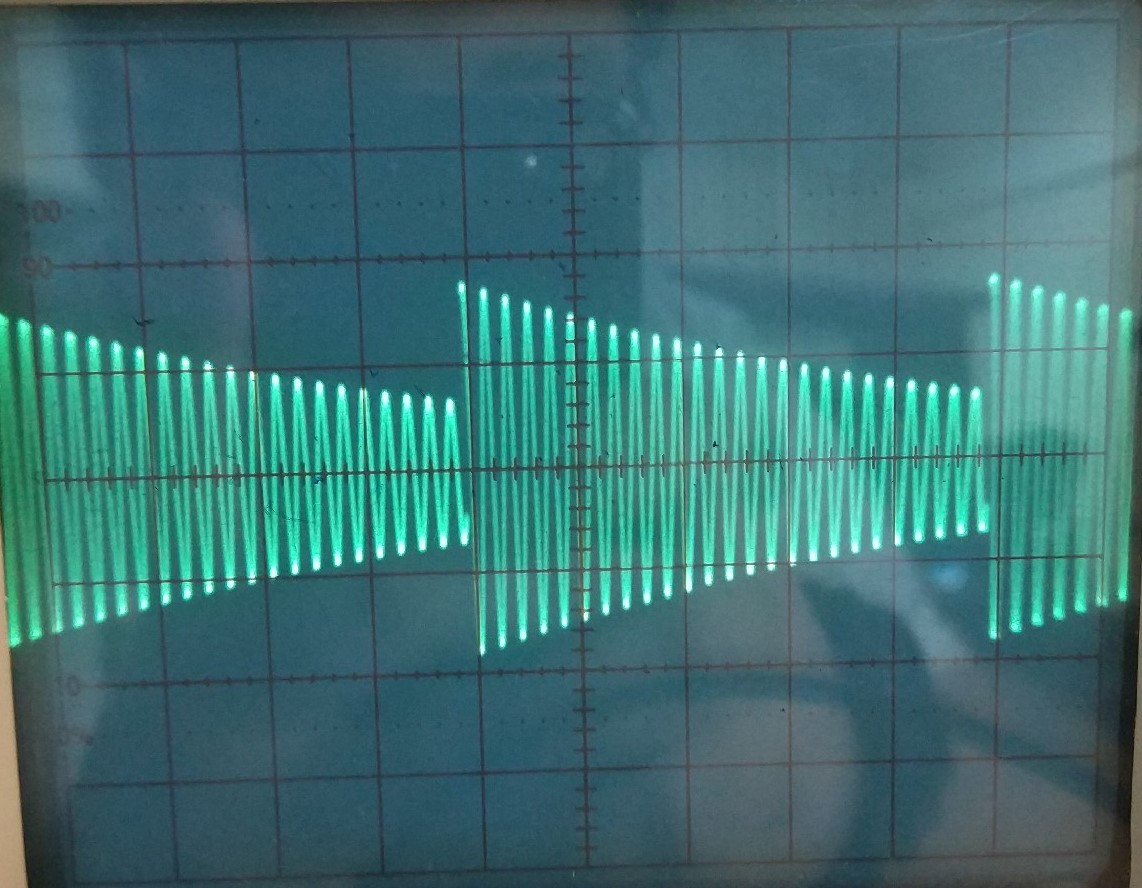
\includegraphics[width = 0.55\textwidth]{part1_1.jpg}
\caption{Колебания в контуре}
\end{center}
\end{figure}

Подбираем частоту развёртски ЭО так, чтобы расстояние $x_0$ между импульсами, поступающими с генератора, занимаело почти весь экран, получено значение $x_0 = 10$ см. 

Теперь, изменяя ёмкость в диапазоне от $0,02$ до $0,09$ мкФ проведем измерения периодов свободных колебаний и сравним их с теоретическими данными по формуле 
\[T = 2 \pi \sqrt{LC}\]

\begin{table}[h!]
\begin{center}
\begin{tabular}{|c|c|c|c|c|c|c|}
\hline
С, нФ & $N$ периодов & $T_{\text{теор}}$, мс & $T_{\text{эксп}}$, мс & $\sigma_T$, мс \\ \hline
20               & 29        & 0,33           & 0,31            & 0,03           \\ \hline
40               & 2         & 0,50           & 0,49            & 0,03           \\ \hline
80               & 3         & 0,67           & 0,66            & 0,03           \\ \hline
120              & 6         & 0,83           & 0,81            & 0,03           \\ \hline
200              & 4         & 1,05           & 1,04            & 0,03           \\ \hline
300              & 3         & 1,33           & 1,31            & 0,04           \\ \hline
400              & 2         & 1,50           & 1,50            & 0,04           \\ \hline
500              & 2         & 1,75           & 1,72            & 0,04           \\ \hline
\end{tabular}
\caption{Таблица данных измерения периода свободных колебаний и сравнение с теорией}
\end{center}
\end{table}

Как видно из таблицы, теоритические данные сходятся с экспериментальными:

\subsection{Измерение критического сопротивления и декремента затухания}

Для начала рассчитаем емкость, при которой частота собственных колебаний контура будет равна $\nu_0 = 5$ кГц.
\[C = \dfrac{1}{4 \pi^2 \nu_0^2 L} \approx 5 \text{нФ}\]
И для значений $L$ и $C$ рассчитаем $R_{crit}$
\[R_{crit} = 2\pi\sqrt{\dfrac{L}{C}} \approx 12,6 \text{кОм}\]
Для этих значений $L$ и $C$ рассчитаем декремент затухания для каждого сопротивления из интервала $(0,1-0,3)R_{crit}$. Из этих данных по формуле 
\[R_{crit} = R_{\Sigma} \sqrt{\left[\dfrac{2\pi}{\theta}\right]^2 + 1}\]
находим $R_{crit}$ запишем все в таблицу. 

\begin{table}[h!]
\begin{center}
\begin{tabular}{|c|c|c|c|c|c|c|c|c|}
\hline
R, Ом & $U_1$, дел & $\sigma_{U_1}$, дел & $U_2$, дел & $\sigma_{U_2}$, дел & $\theta$ & $\sigma_{\theta}$ & $R_{crit}$, Ом & $\sigma_{R_{crit}}$, Ом \\ \hline
1200  & 4          & 0,2                 & 2,1        & 0,2                 & 0,64     & 0,07              & 11800          & 1000                    \\ \hline
1500  & 4          & 0,2                 & 1,8        & 0,2                 & 0,80     & 0,10              & 11900          & 1300                    \\ \hline
1800  & 4          & 0,2                 & 1,6        & 0,2                 & 0,92     & 0,12              & 12500          & 1600                    \\ \hline
2100  & 4          & 0,2                 & 1,3        & 0,2                 & 1,1      & 0,2               & 11900          & 1400                    \\ \hline
2400  & 4          & 0,2                 & 1,1        & 0,2                 & 1,3      & 0,2               & 11900          & 1300                    \\ \hline
2700  & 4          & 0,2                 & 1          & 0,2                 & 1,4      & 0,3               & 12500          & 1000                    \\ \hline
3000  & 4          & 0,2                 & 0,8        & 0,2                 & 1,6      & 0,4               & 12000          & 1300                    \\ \hline
3300  & 4          & 0,2                 & 0,7        & 0,2                 & 1,7      & 0,5               & 12300          & 1600                    \\ \hline
\end{tabular}
\caption{Таблица измерения $R_{crit}$}
\end{center}
\end{table}

В итоге мы получаем, что $R_{crit} = (12,1 \pm 1,8)$ кОм.

Так же мы можем получить $R_{crit}$ просто подбором, добиваясь подобной картины

\begin{figure}[h]
\begin{center}
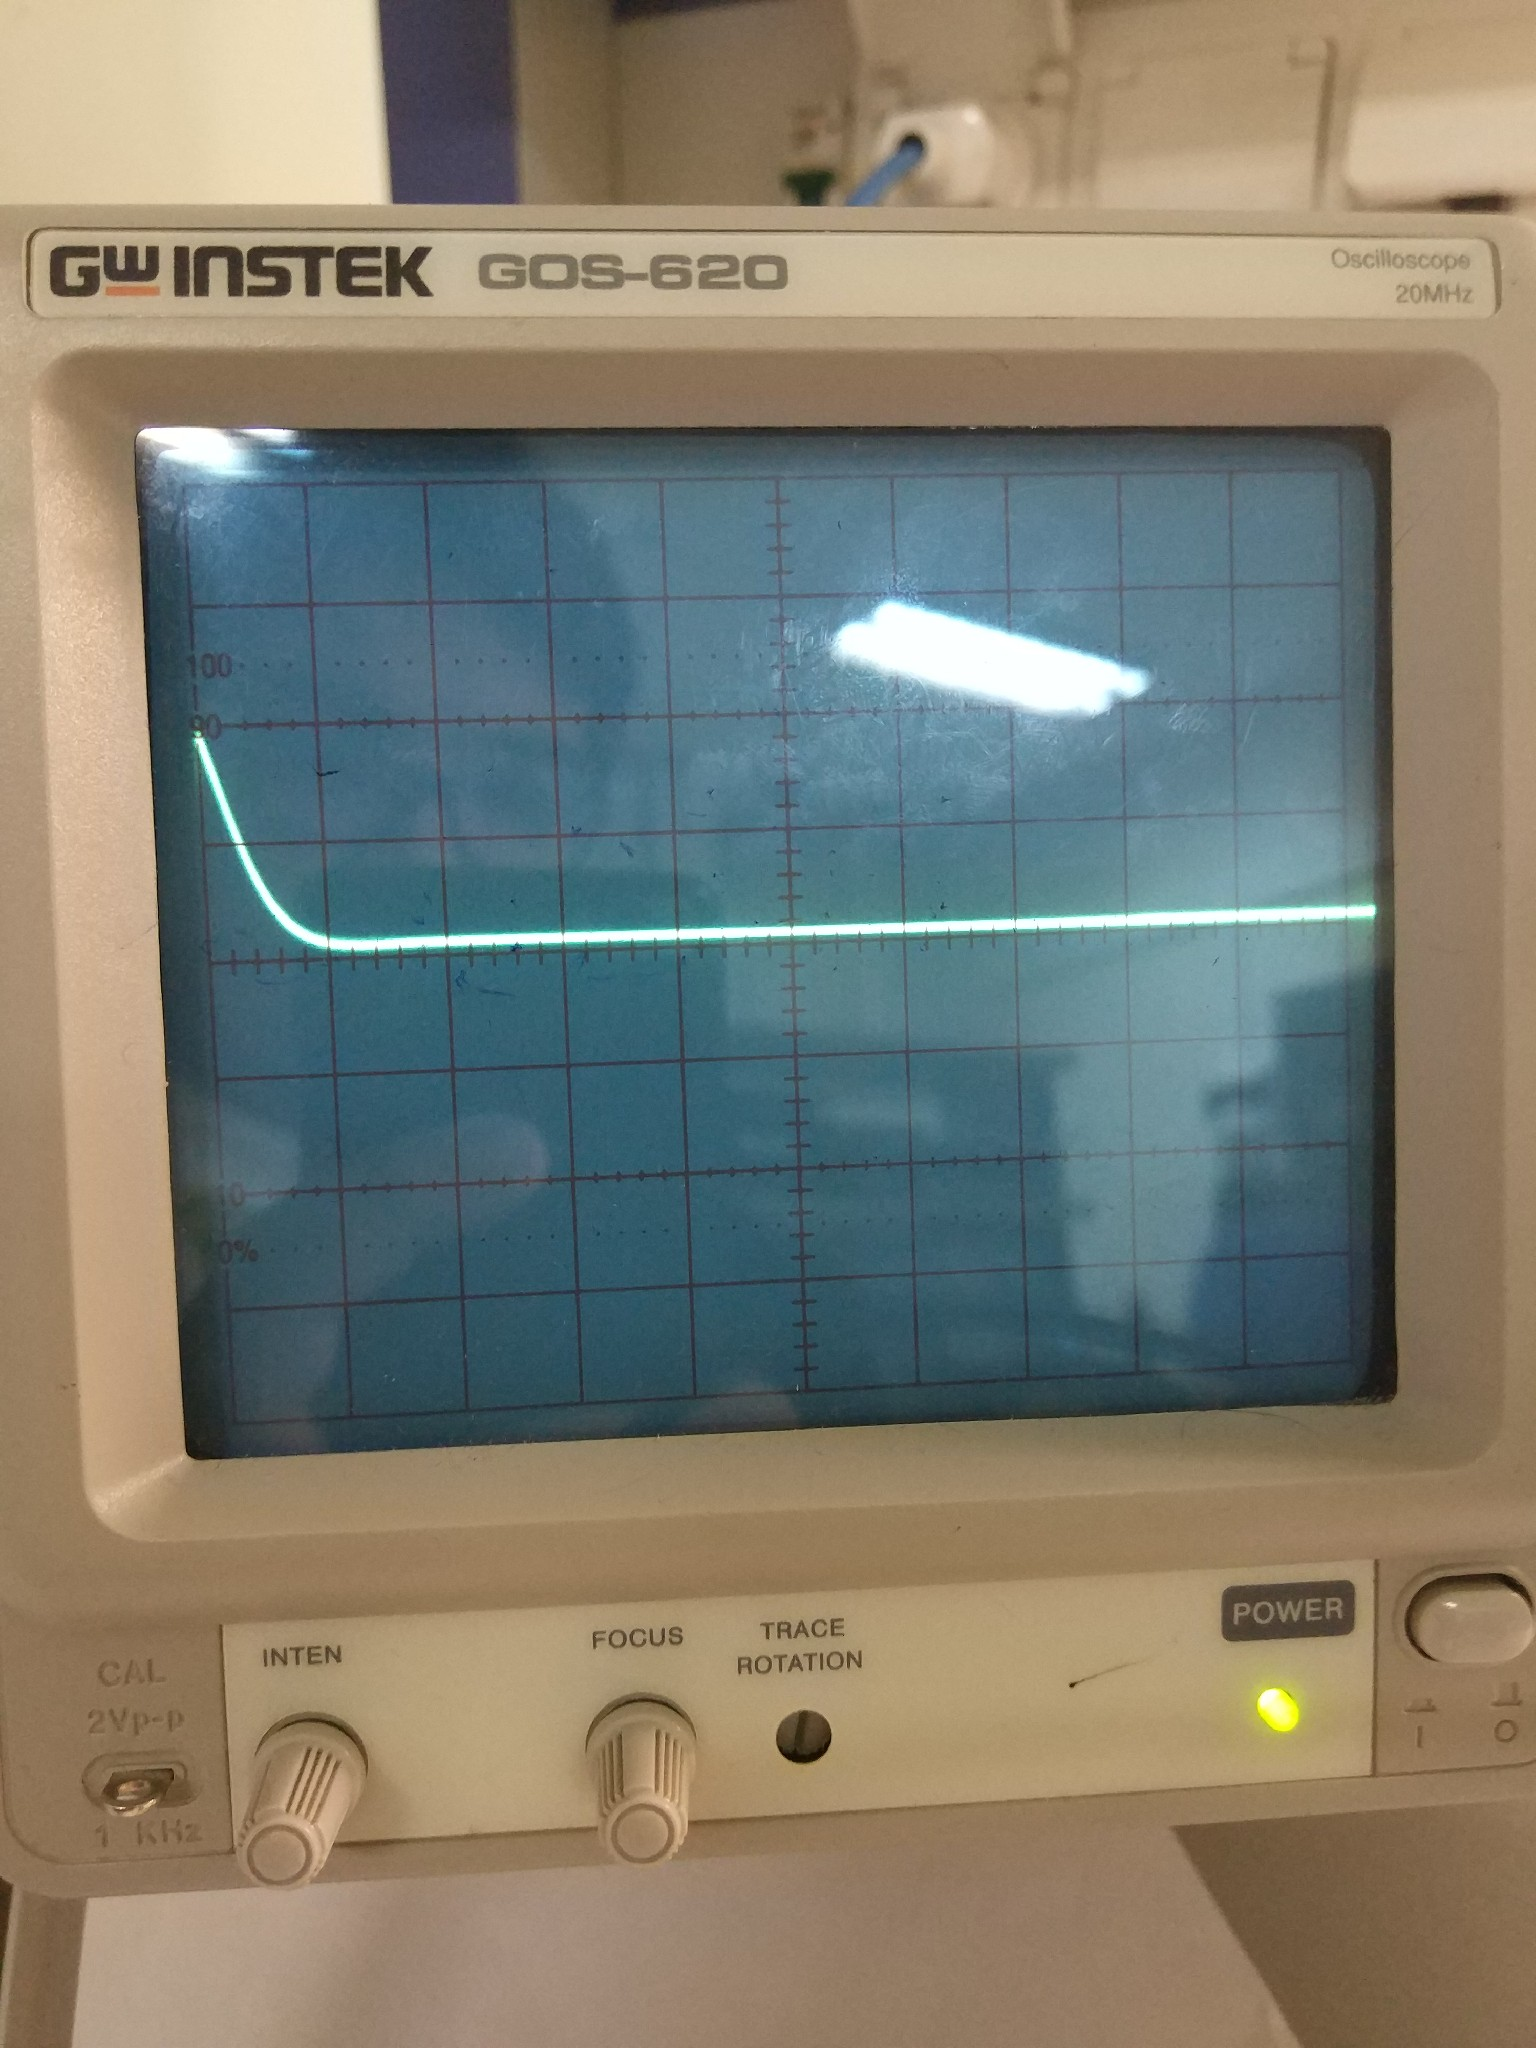
\includegraphics[width = 0.4\textwidth]{2.jpg}
\caption{Затухание колебаний}
\end{center}
\end{figure}

Подбирая мы получаем, что $R_{crit} \approx 12$ кОм.
\newpage
\subsection{Свободные колебания на фазовой плоскости}
Рассмотрим свободные колебания на фазовой плоскости, для этого подключим место соединения катушки индуктивности и магазина сопротивлений к выходу $X$ и включим на осциллографе канал $X-Y$. В итоге мы получаем картинку на экране как на рисунке ниже. 
\begin{figure}[h!]
\begin{center}
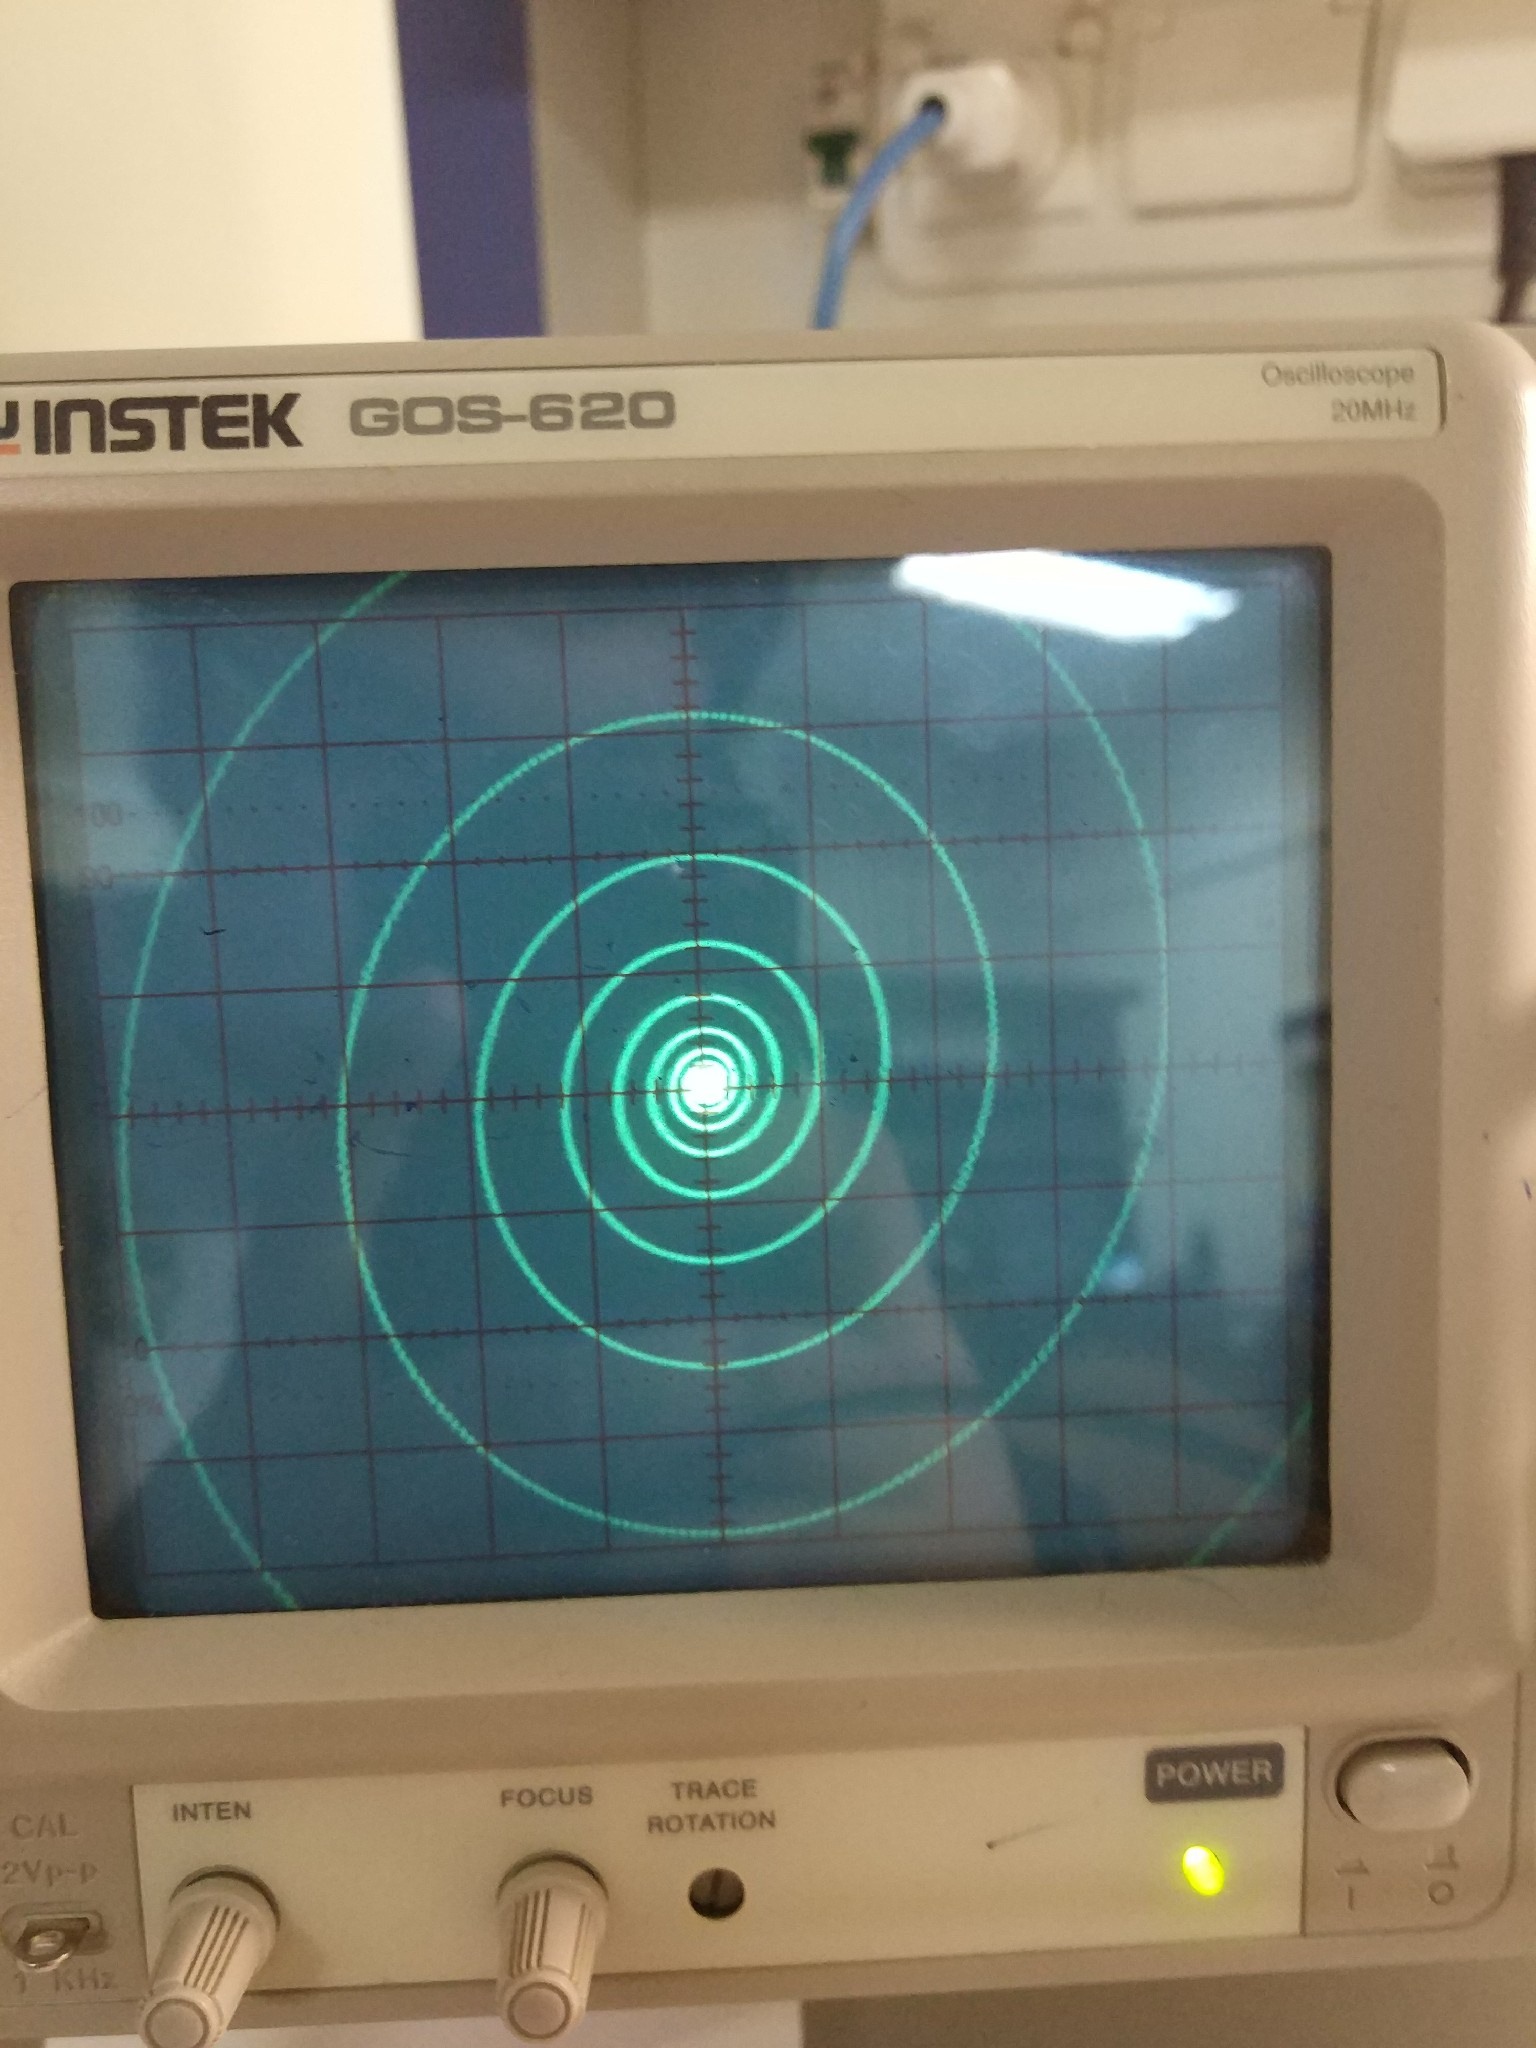
\includegraphics[width = 0.6\textwidth]{1.jpg}
\caption{Фазовая диаграмма для свободных колебаний}
\end{center}
\end{figure}

Для фазовой диаграммы для двух значений посчитаем так же декремент затухания

\begin{table}[h!]
\begin{center}
\begin{tabular}{|c|c|c|c|c|}
\hline
$R$, Ом &$U_1$, дел & $U_2$, дел & $\theta$ & $\sigma_{\theta}$ \\ \hline
1800 &4,1        & 1,6        & 0,94    & 0,15              \\ \hline
3000& 3          & 0,5        & 1,8     & 0,2              \\ \hline
\end{tabular}
\caption{Декремент затухания для фазовой диаграммы}
\end{center}
\end{table}

Видим, что мы получили такой же декремент затухания как и при его подсчете из графика колебаний.
\subsection{Добротность свободных колебаний в контуре}
Добротность можно найти по формуле 
\[Q = \dfrac{\pi}{\theta}\]
Найдем ее для $R_{max} = 3$ кОм и для $R_{min} = 1,8$ кОм из графика и фазовой диаграммы. Итоговые результаты запишем в таблицу.

Так же добротность можно найти и из теоретических соображений по формуле
\[Q = \dfrac{1}{R}\sqrt{\dfrac{L}{C}}\]

Результаты так же занесем в таблицу, и в итоге мы получаем эту таблицу со всеми данными из данного эксперимента, по которой мы можем сравнить все полученные значения


\section{Вывод}
Как видно из таблицы 5, наилучший способ измерения добротности --- с помощью графика, потому что получаются наиболее близкие значения с меньшими погрешностями. Так же из графика видно, что $R_{crit}$ лучше измеряется при более высоком сопротивлении в контуре. 

\section{Литература}
\begin{enumerate}
\item \textbf{Лабораторный практикум по общей физике:} Учебное пособие. В трех томах. Т. 2. Электричество и магнетизм /Гладун А.Д., Александров Д.А., Берулёва Н.С. и др.; Под ред. А.Д. Гладуна - М.: МФТИ, 2007. - 280 с.
\item \textbf{Дополнительное описание лабораторной работы 3.2.4}: Свободные колебания в электрическом контуре; Под ред. МФТИ, 2018 г. - 4 с.
\end{enumerate}

					\end{document}